\section{results}\label{sec:results}
\subsection{Generation results}\label{subsec:generation-results}
This section will present the results of generating the VOID description and show how the size of the database affects the generation time. First, how the results were measured will be explained; then, the results will be presented and discussed.

The results were made by measuring the generation time for a VOID description for different database sizes. The database started at 1 million triples and was incremented by 10.000 triples up to 10.000.000. A VOID description was generated for each increment for the database, and the time it took to generate it was measured in ms. This was done ten times to ensure the results would be reliable. From this, a graph could be made, and a linear regression could be made to show the trend of the generation time. This help to show how much the time to generate a VOIID description increases as the database size increases.

A graph of the standard derivation of the results can be seen in \autoref{fig:generate-dbsize-all}, which shows the size of the database along the x-axis and the generation time in ms on the y-axis. Each point in the graph has a span, the standard derivation of the results. From the graph, it is clear to see that there is a trend that the data follows. As the database size increases, so does the time it takes to generate a VOID description; the time increases linearly with the database size. Though there is a strange trend when the database reaches the size above 8.000.000 triples, the standard derivation of the results suddenly decreases. To better understand why this happens, we can show a graph over all ten runs and, from this, see if there is anything that could indicate why the sudden decrease happens. In \autoref{fig:generate-dbsize-10-runs-all}, we can see the results of all ten runs. Certain outliers deviate significantly from others. This is most likely because the computer running the measurements was in use during the first few runs. This has likely affected the results and caused the outliers. This can be even more seen when sorting these outliers out in \autoref{fig:generate-dbsize-10-runs-good}. In this graph, all the results are much more similar, showing that, when generating the results, it was susceptible to any other activity happening on the machine, thereby creating outliers. So by generating a new graph with the outliers removed, we can see that the standard derivation of the results is much more stable and still follows the same trend as before.

From this, we can gather that the time it takes to generate a VOID description for a database linearly increases as the database size increases. This is expected as the more triples the database has, the more triples the script has to process and the longer it will take to generate the VOID description.


\subsection{Update results}\label{subsec:update-results}
As in \autoref{subsec:generation-results}, how the results were measured will be explained; then, the results will be presented and discussed.

The results for updating the VOID description contained three parameters: time, query size, and database size. The query size was measured for updating the VOID description and not for generating it because the query size was not affecting generation, as the generation is purely based on what is in the database.

The results were made by measuring the time it took to update the VOID description for database and query sizes. As in \autoref{subsec:generation-results}, the database started at 1 million triples and incremented by 10.0000 triples up to 10.000.000. The query size starts at one triple and increases by 1.000 until reaching 8.001, whereafter the database increments by 10.000, and the query size starts at one again. For each change in the query size, a measurement is made for how long it takes to update the VOID description. Since nine additional measurements were made for each database size increment, there was a much more significant amount of data when compared to the measurements for \autoref{subsec:generation-results}. It is important to note that the query was never inserted into the database, which is why it did not directly impact the database size and why the database size was not incremented by 1.000 for each query size increment.

As with \autoref{subsec:generation-results} there was some data that was impacted by the computer being in use during the measurements. This can be seen in figure \autoref{fig:update-querysize-all}, where there are some outliers that deviate significantly from the rest of the data. Because of the outliers, we are mainly interested in the data that was generated without the computer being in use, as this data is more reliable, as can be seen in \autoref{fig:update-querysize-good}.

With the results for updating the VOID description, \autoref{fig:update-querysize-dbsize-good} could be made, which shows query size along the x-axis, the database size along the y-axis, and the time along the z-axis. From this graph, it is clear to see that there is a trend that the data follows. The query size has a significant impact on the time it takes to update the VOID description, and it seems that the database size also impacts the times, but if it does, it is not as significant as the query size. Meaning that as the amount of new data that is to be inserted in the database increases, so does the time it takes to update the VOID description. Which is to be expected, as the more data that is inserted, the more data the script has to process and the longer it will take to update the VOID description. All the data that is inserted is new data, meaning that currently it is unknown if updating existing data will have a significant impact on the time it takes to update the VOID description. This is something that could be tested in the future, but we assume that it will not have a significant impact on the time it takes to update the VOID description.
\task{Consider making an experiment that tests for updating new vs. updating existing data.}

Additionally a 2d graph was made to more clearly display the impact of database size and query size. In \autoref{fig:update-querysize-dbsize-good} we can see that the size of the database has a minor effect on the time to update, but the query size is the main factor in the time it takes to update the VOID description. This is to be expected, as the more information the query contains, the more information the script has to process, and the longer it will take to update the VOID description, and since VOID description is not created from scratch, but instead updated, the size of the database does not have a significant impact on the time it takes to update the VOID description. There is an unexpected trend in the graph, where the time it takes to update the VOID description suddenly decreases, when the database is almost 10.000.000 triples. It is not known for sure what the cause of this effect was, but it is suspected that the end of the data file where the triples are taken from, has triples that contain significantly fewer characters than the rest of the file, which could explain the sudden decrease in time.

From these finding we can gather that the time it takes to update a VOID description is heavily impacted by the size of the query (the amount of characters in the query) that is being inserted, and not so much the size of the database.


\subsection{Update and generation comparison}\label{subsec:update-generation-comparison}
This section will compare the two methods that have been measured and described, showing their differences and when it makes sense to use one over the other. The comparison will be based on combining the results from \autoref{subsec:generation-results} and \autoref{subsec:update-results}.

The following figure \autoref{fig:comparison-generation-vs-update} shows a 2d graph of the impact of database size on the time it takes to generate a VOID description and the time it takes to update a VOID description. Since generating a VOID description is greatly affected by the size of the database, it can be seen that the time it takes to generate a VOID description increases significantly faster than the time it takes to update a VOID description. In comparison, the database size barely affects the nine update measurements for each query size. From this, it can be gathered that the larger the database is, the more it makes sense to update the VOID description instead of generating it from scratch, but with a smaller database, it makes more sense to generate the VOID description from scratch.


\begin{figure*}
    \centering
    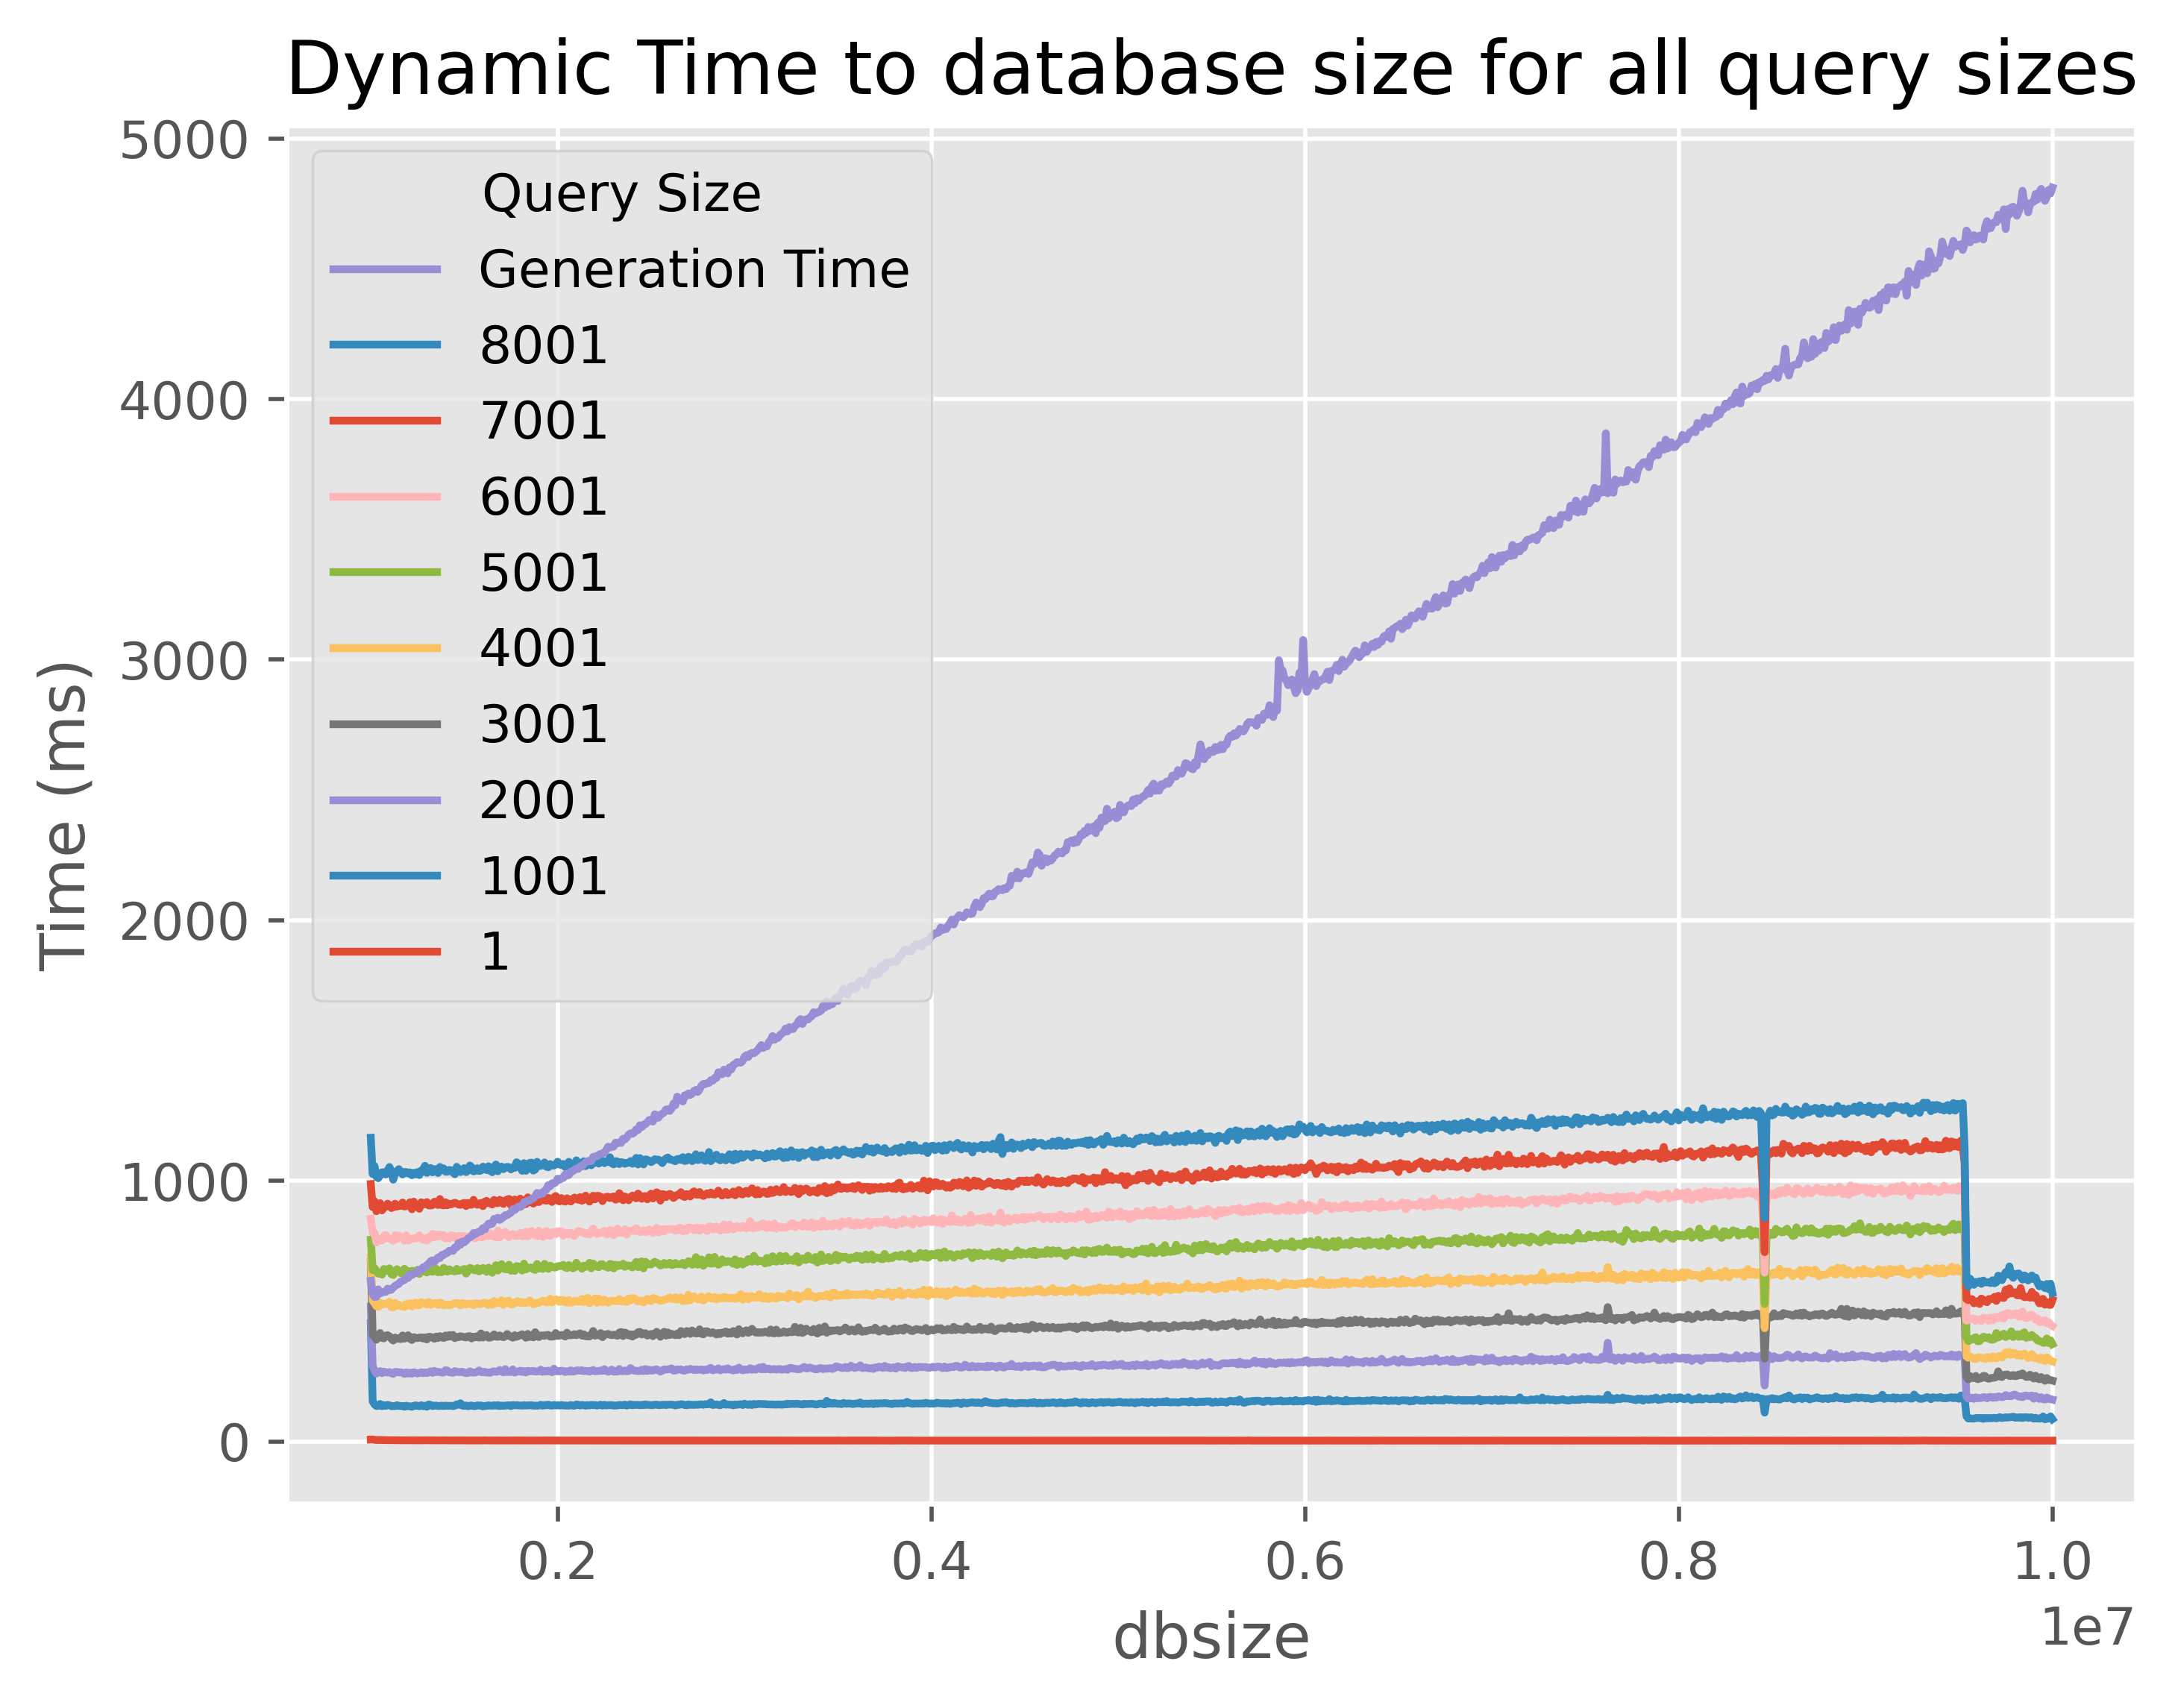
\includegraphics[width=0.8\textwidth]{figures/comparison-Generation-vs-Update.png}
    \caption{Comparison between the time it takes to generate a VOID description and the time it takes to update a VOID description, based on database size.}
    \label{fig:comparison-generation-vs-update}
\end{figure*}

\begin{figure}
    \centering
    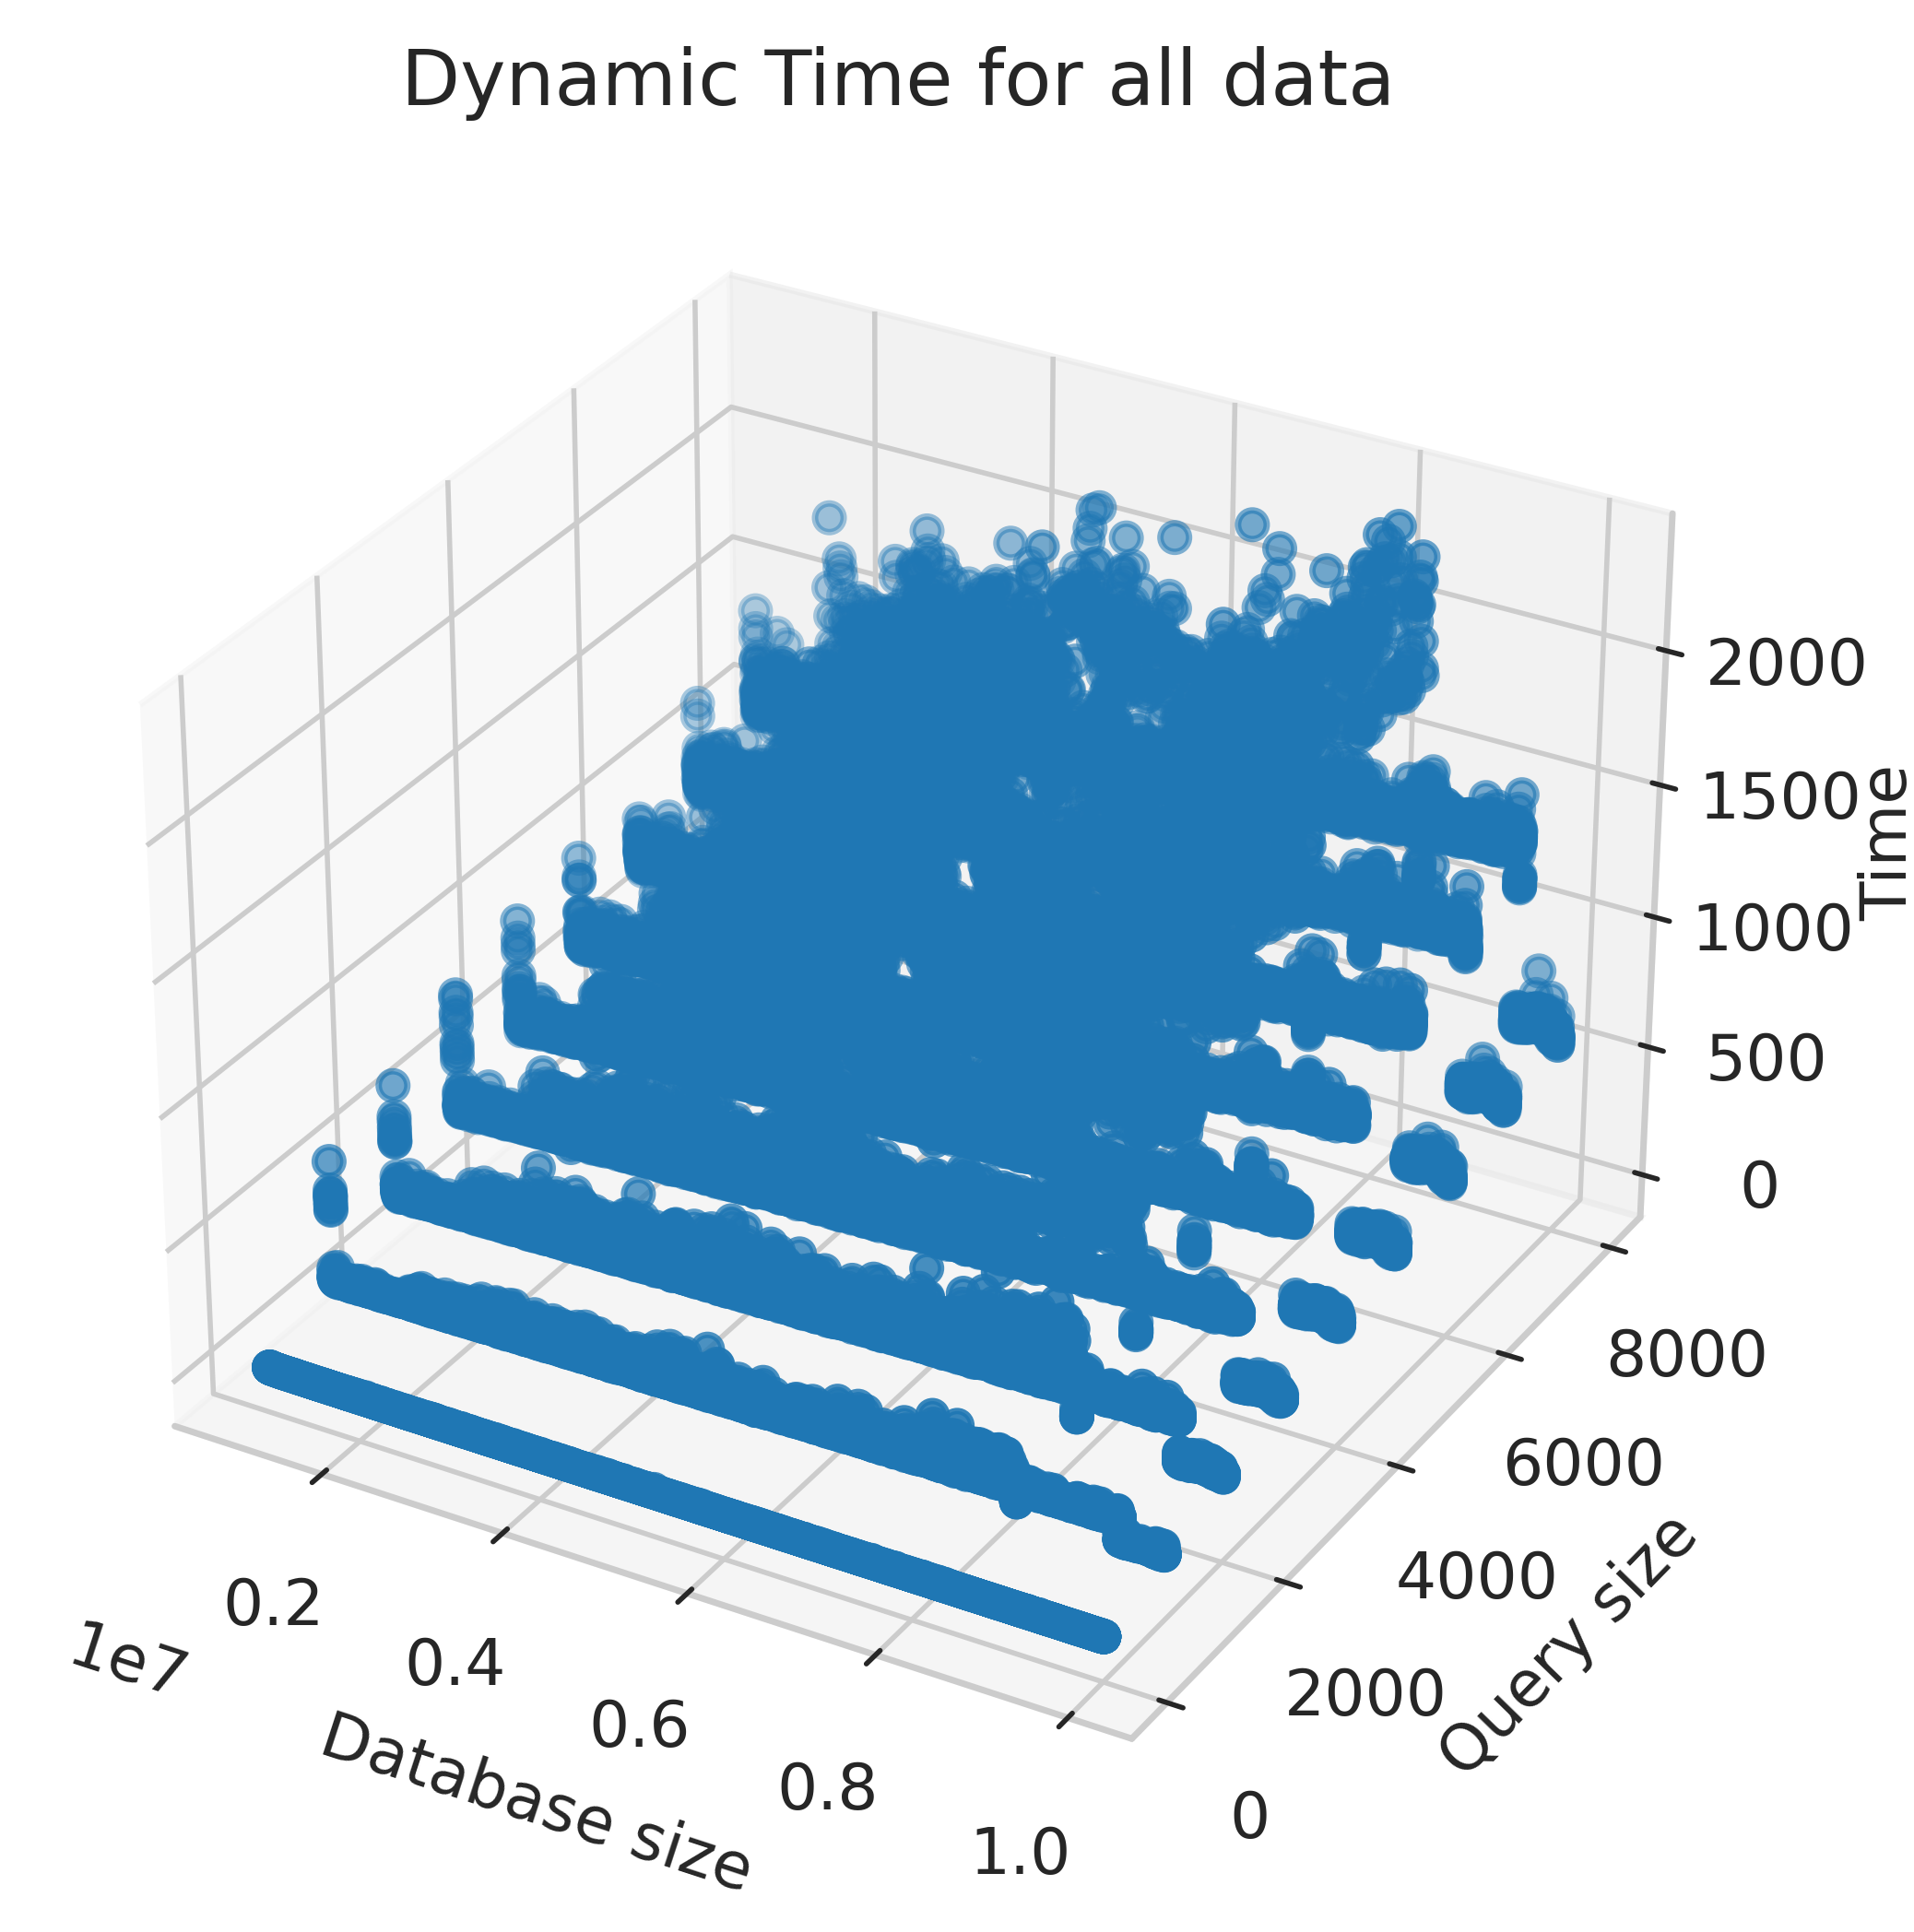
\includegraphics[width=0.8\columnwidth]{figures/dynamic-time-for-all.png}
    \caption{3D graph showing the impact of query size and database size on the time it takes to update a VOID description, containing all the data.}
    \label{fig:update-querysize-dbsize-all}
\end{figure}

\begin{figure}
    \centering
    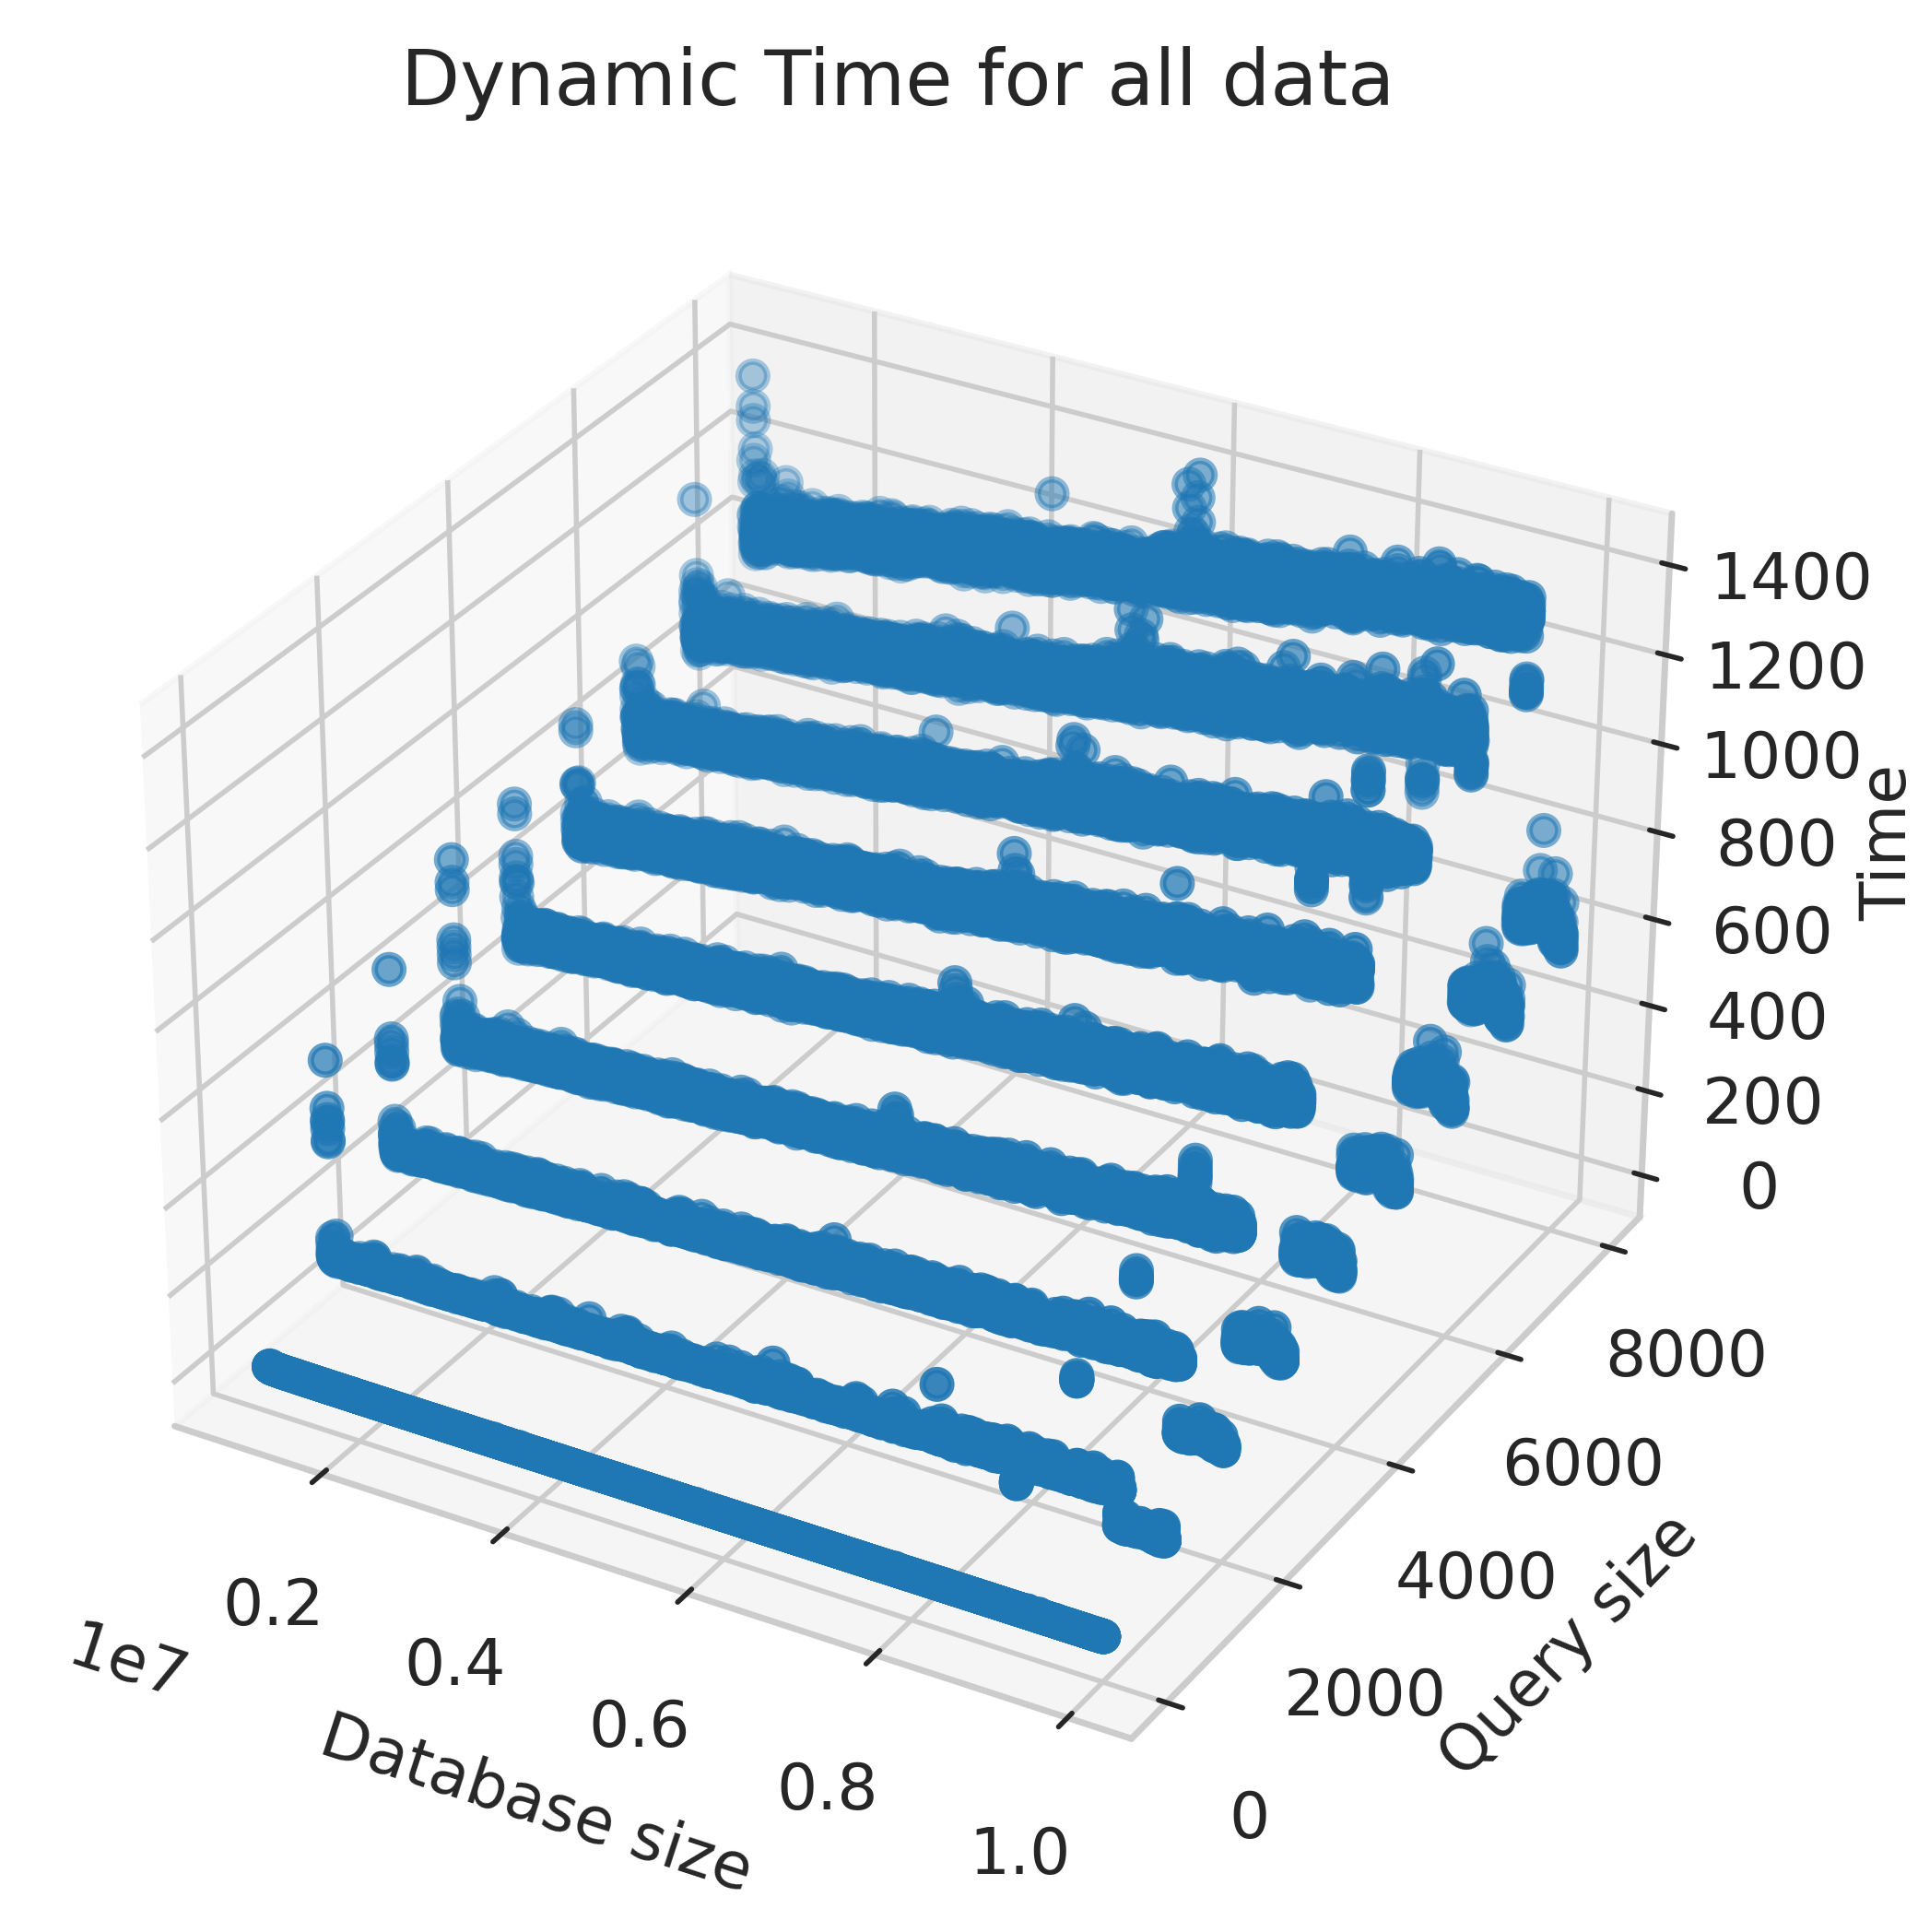
\includegraphics[width=0.8\columnwidth]{figures/dynamic-time-for-all-good.png}
    \caption{3D graph showing the impact of query size and database size on the time it takes to update a VOID description, containing only the good data.}
    \label{fig:update-querysize-dbsize-good}
\end{figure}

\begin{figure}
    \centering
    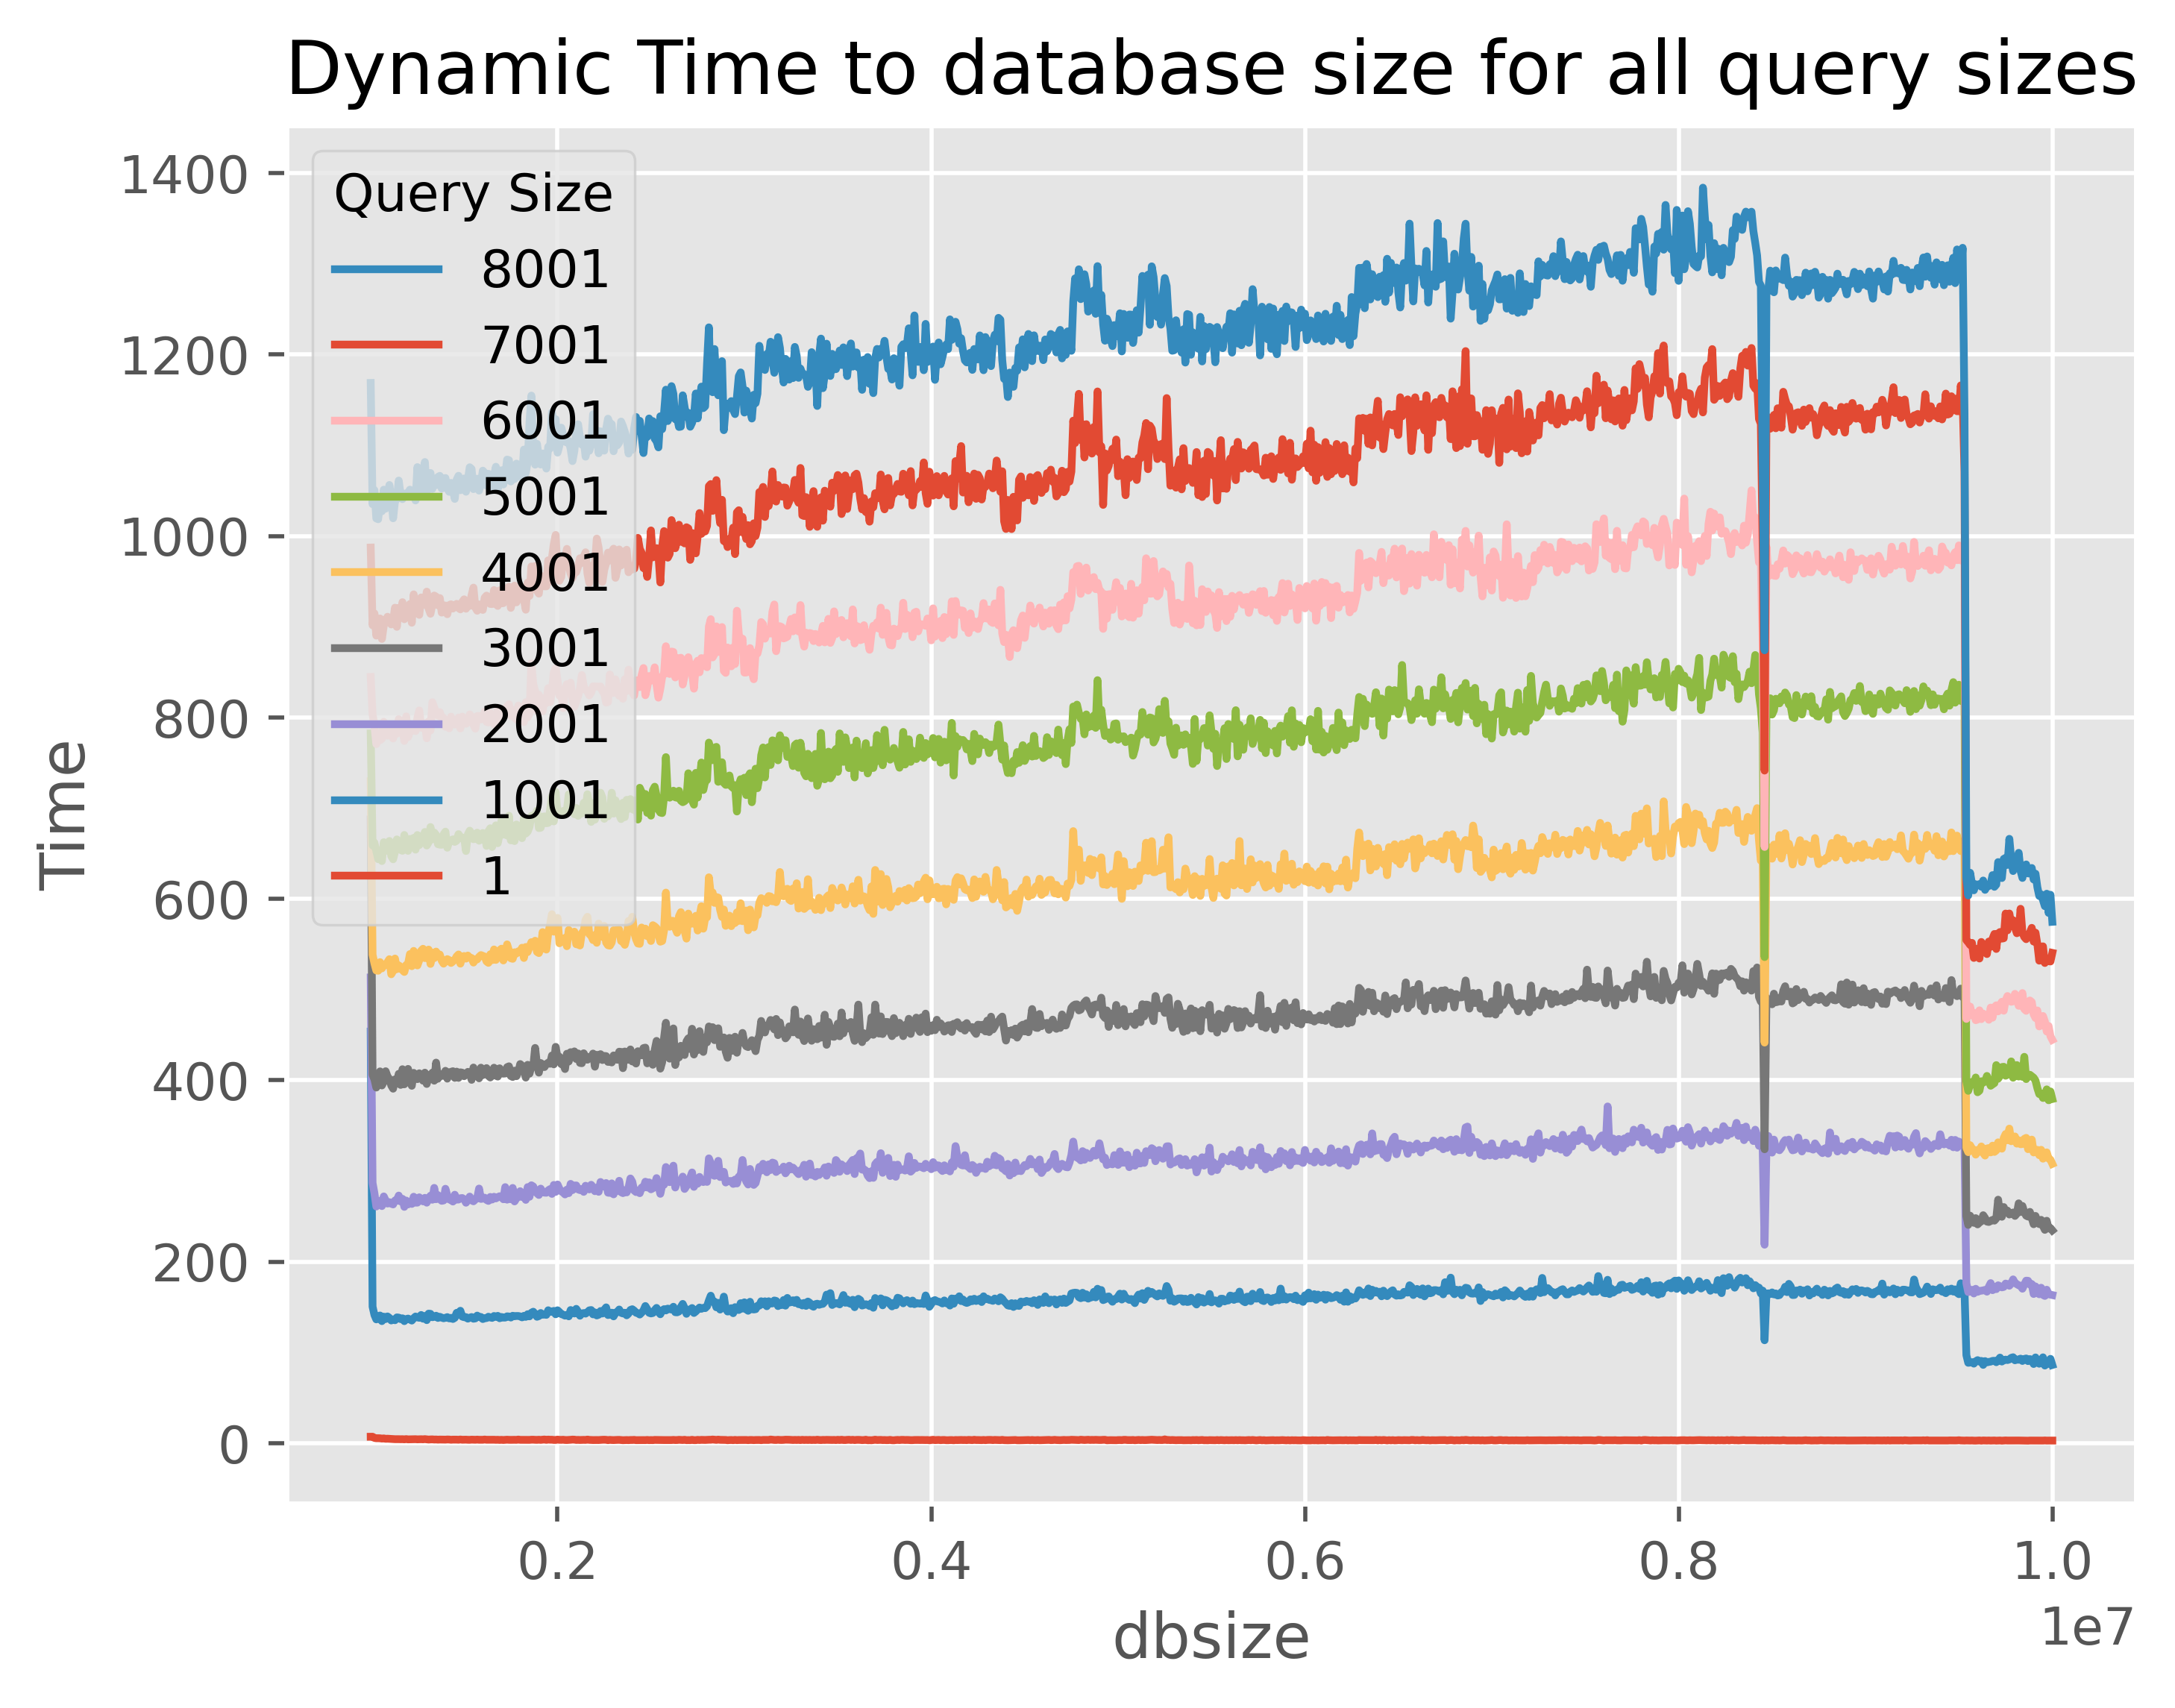
\includegraphics[width=0.8\columnwidth]{figures/dynamic-time-query-size-all.png}
    \caption{2D graph showing the impact of query size and database size on the time it takes to update a VOID description, containing all the data.}
    \label{fig:update-querysize-all}
\end{figure}

\begin{figure}
    \centering
    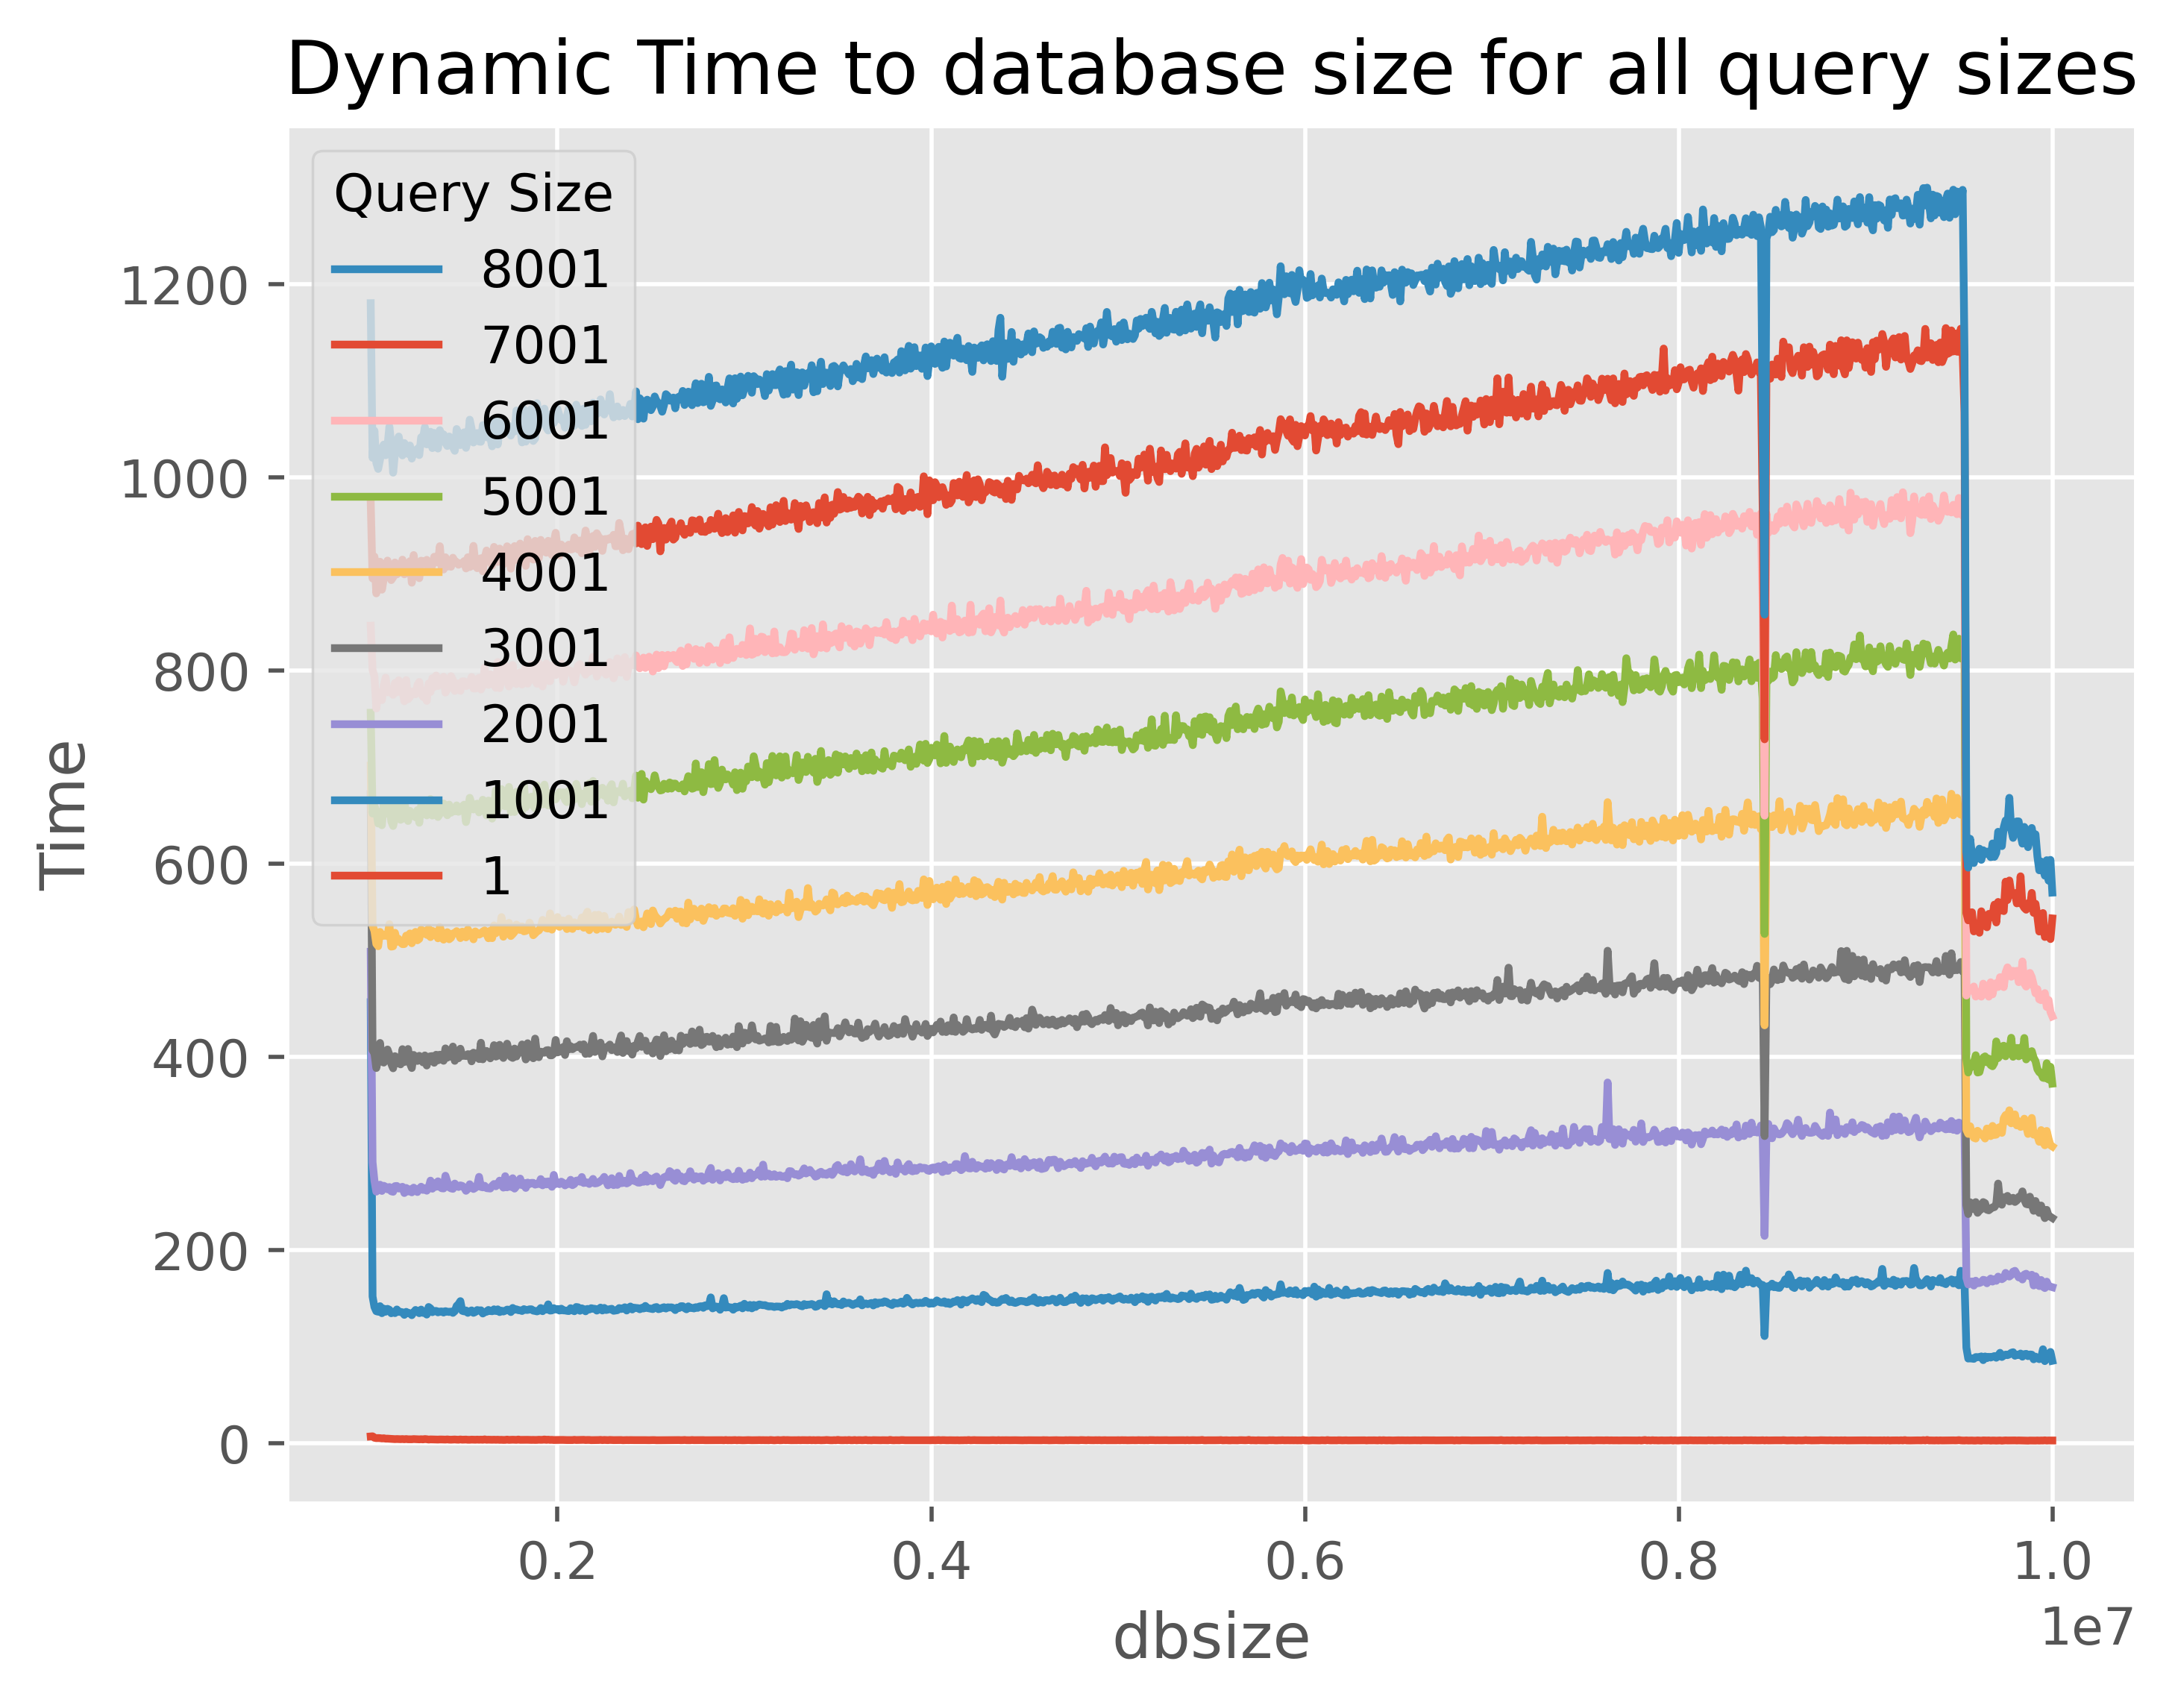
\includegraphics[width=0.8\columnwidth]{figures/dynamic-time-query-size-good.png}
    \caption{2D graph showing the impact of query size and database size on the time it takes to update a VOID description, containing only the good data.}
    \label{fig:update-querysize-good}
\end{figure}

\begin{figure}
    \centering
    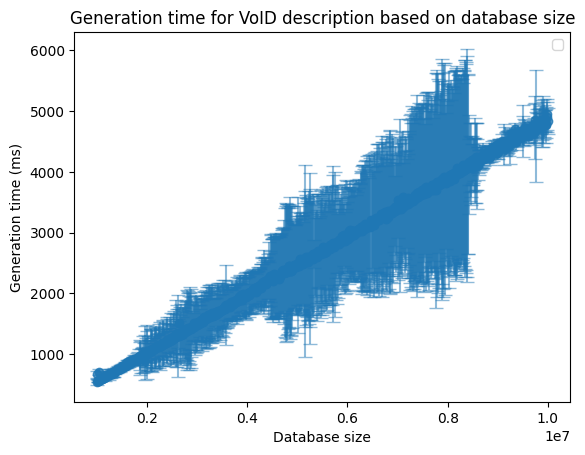
\includegraphics[width=0.8\columnwidth]{figures/generation-results-graph.png}
    \caption{2D graph showing the standard deriviation impact of database size on the time it takes to generate a VOID description. Containing all the data.}
    \label{fig:generate-dbsize-all}
\end{figure}

\begin{figure}
    \centering
    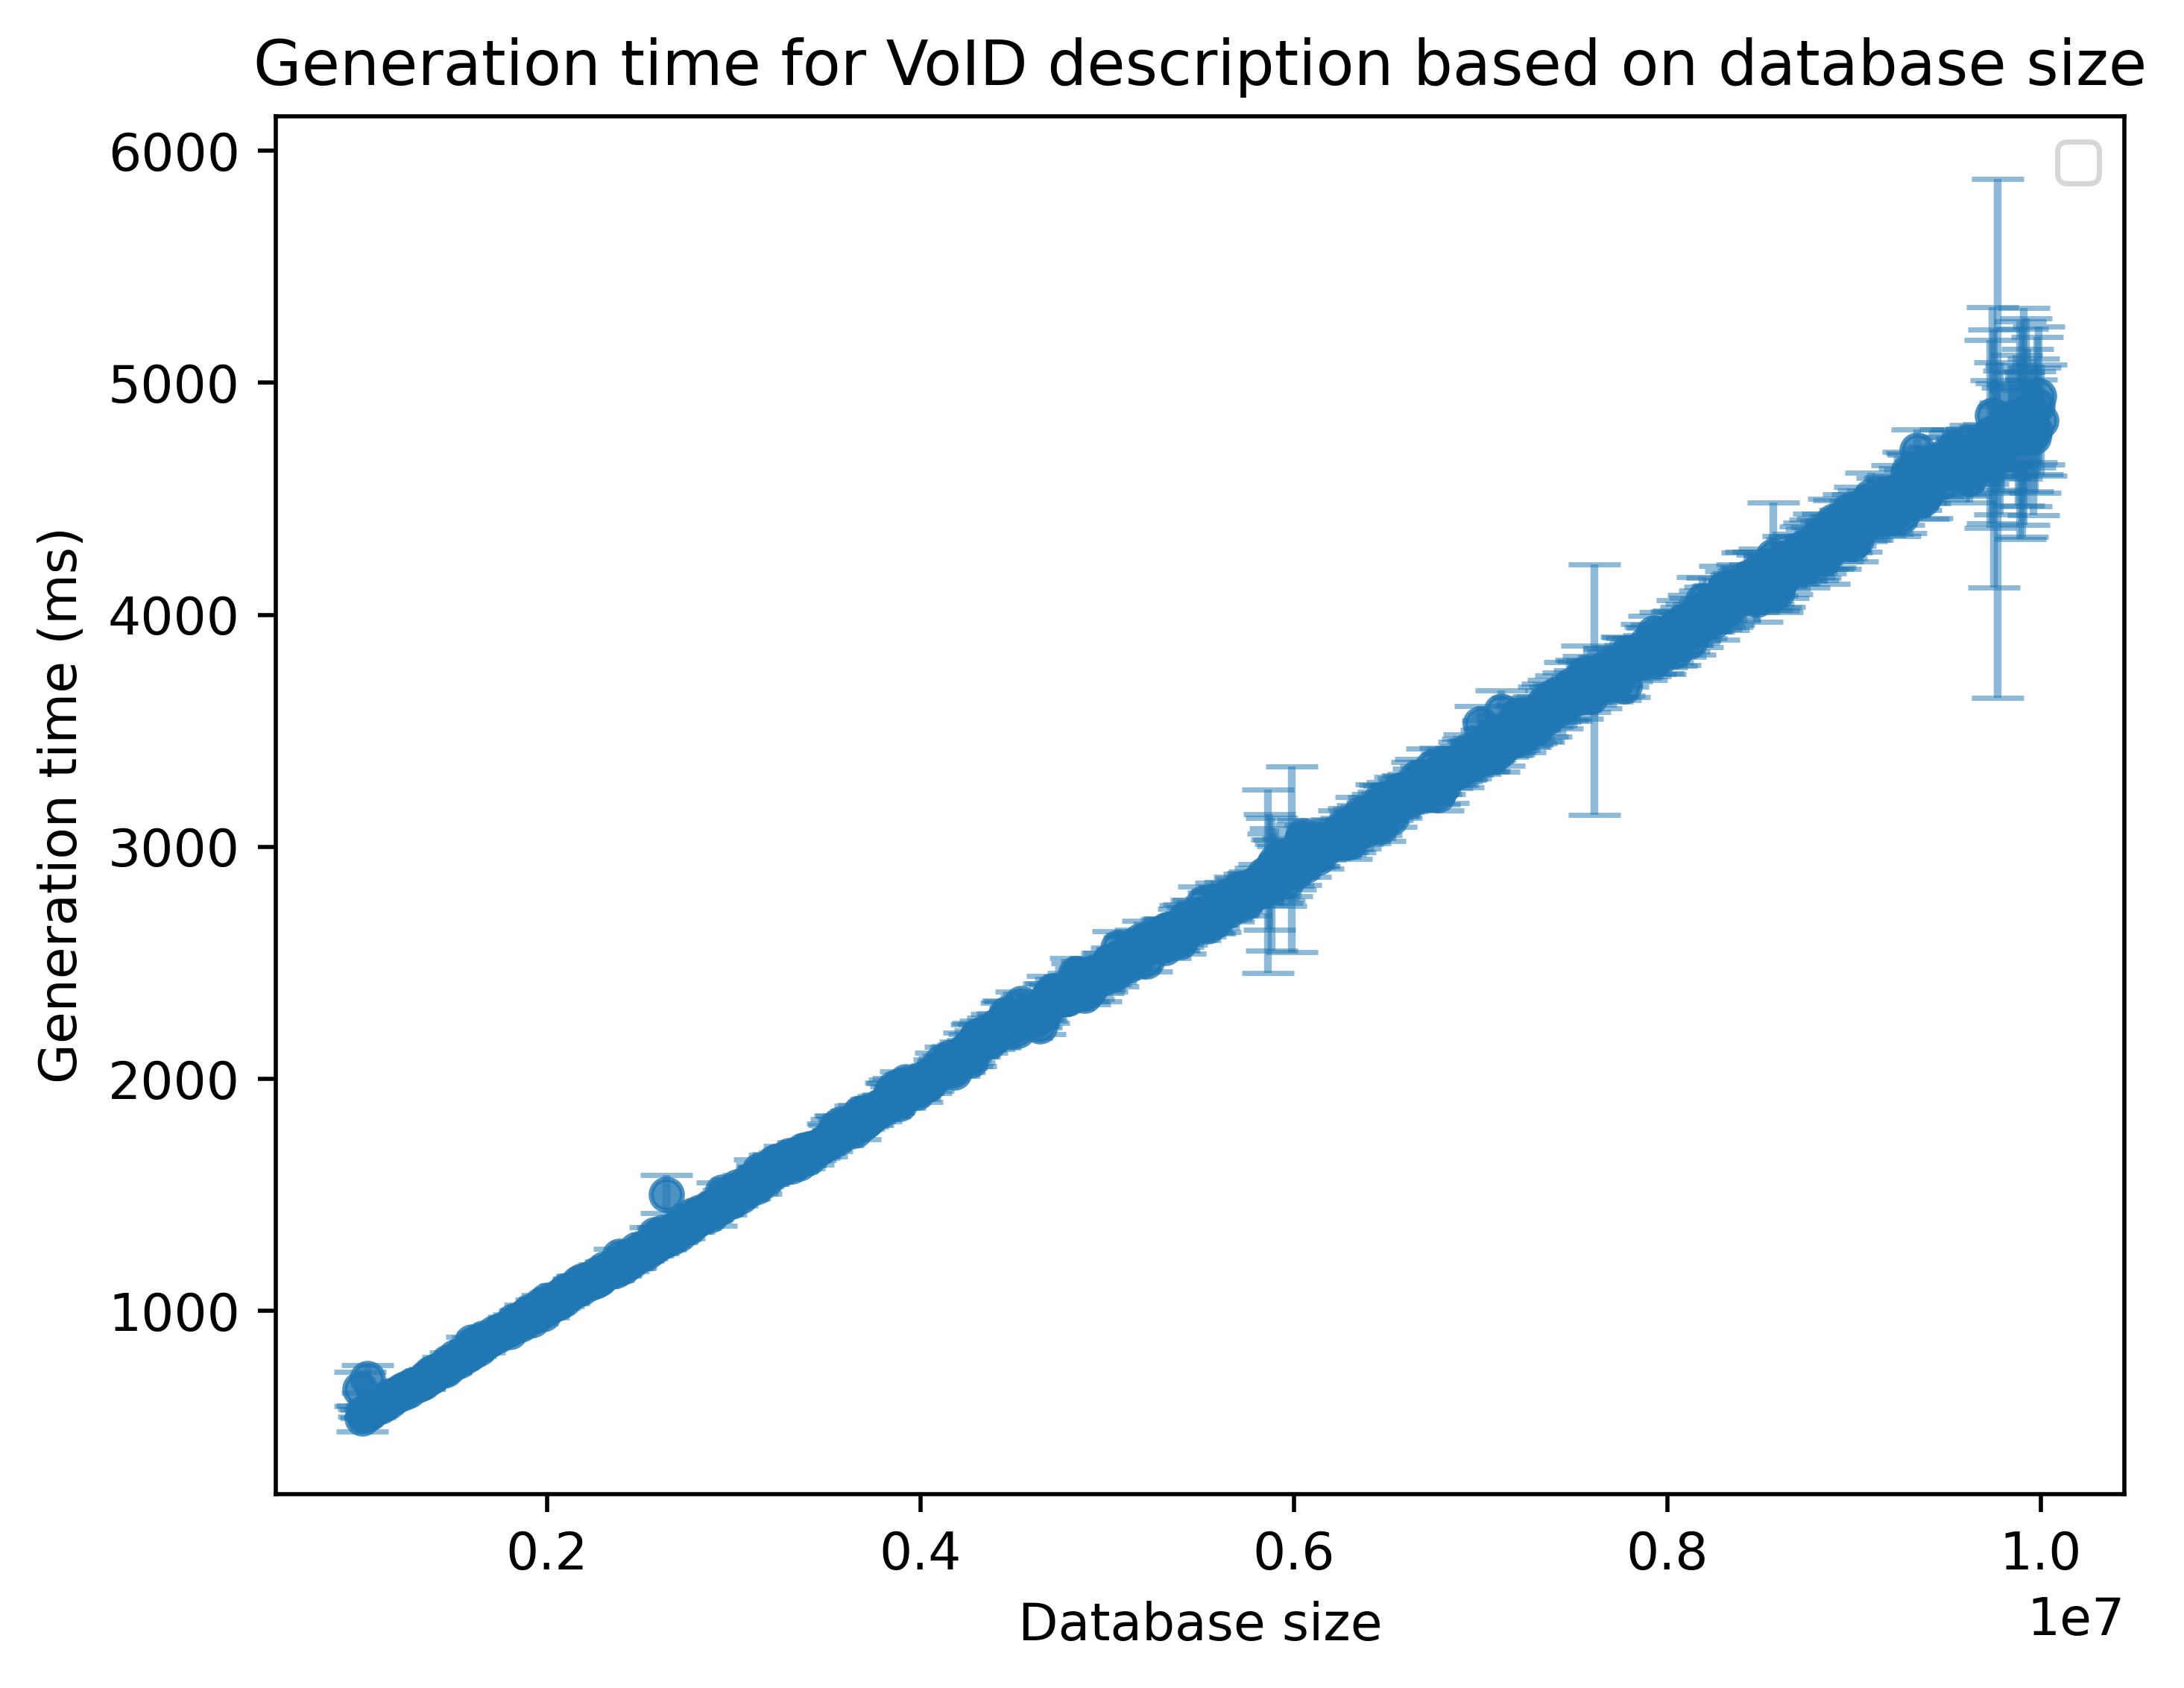
\includegraphics[width=0.8\columnwidth]{figures/generation-results-graph-good.png}
    \caption{2D graph showing the standard deriviation impact of database size on the time it takes to generate a VOID description. Containing only the good data.}
    \label{fig:generate-dbsize-good}
\end{figure}

\begin{figure}
    \centering
    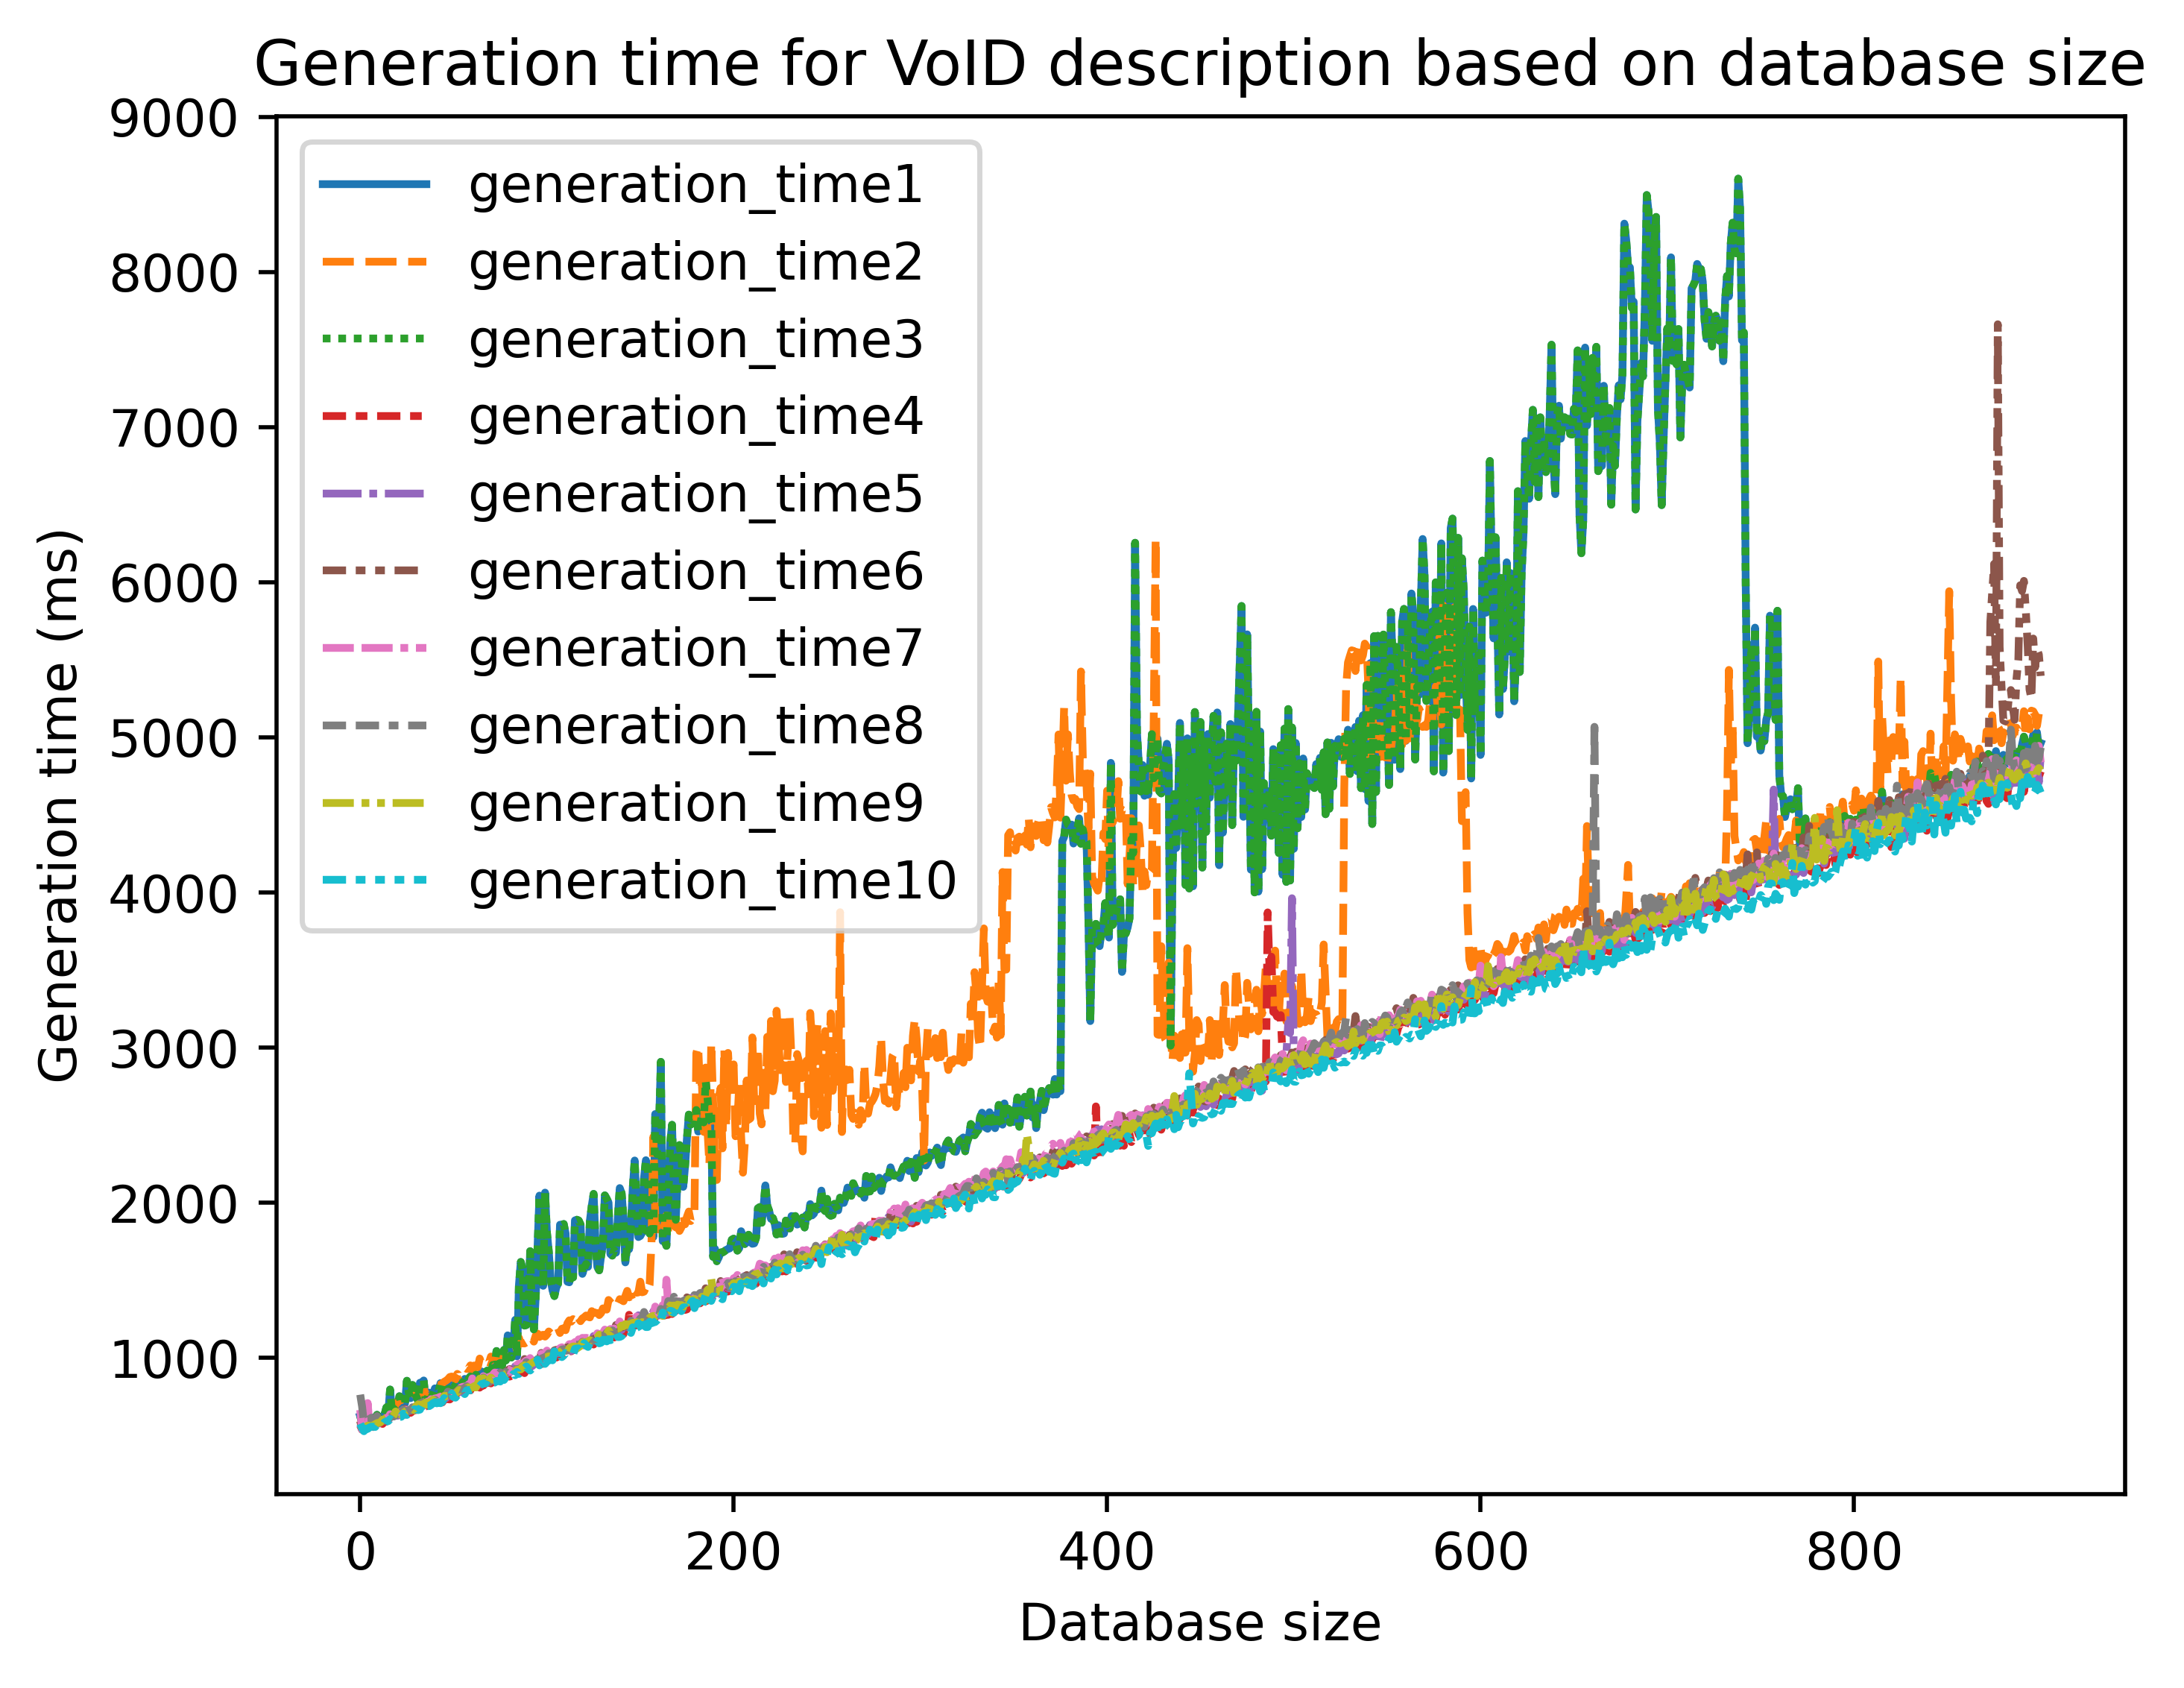
\includegraphics[width=0.8\columnwidth]{figures/generation-results-graph-all.png}
    \caption{2D graph showing each runs impact of database size on the time it takes to generate a VOID description. Containing all the data.}
    \label{fig:generate-dbsize-10-runs-all}
\end{figure}

\begin{figure}
    \centering
    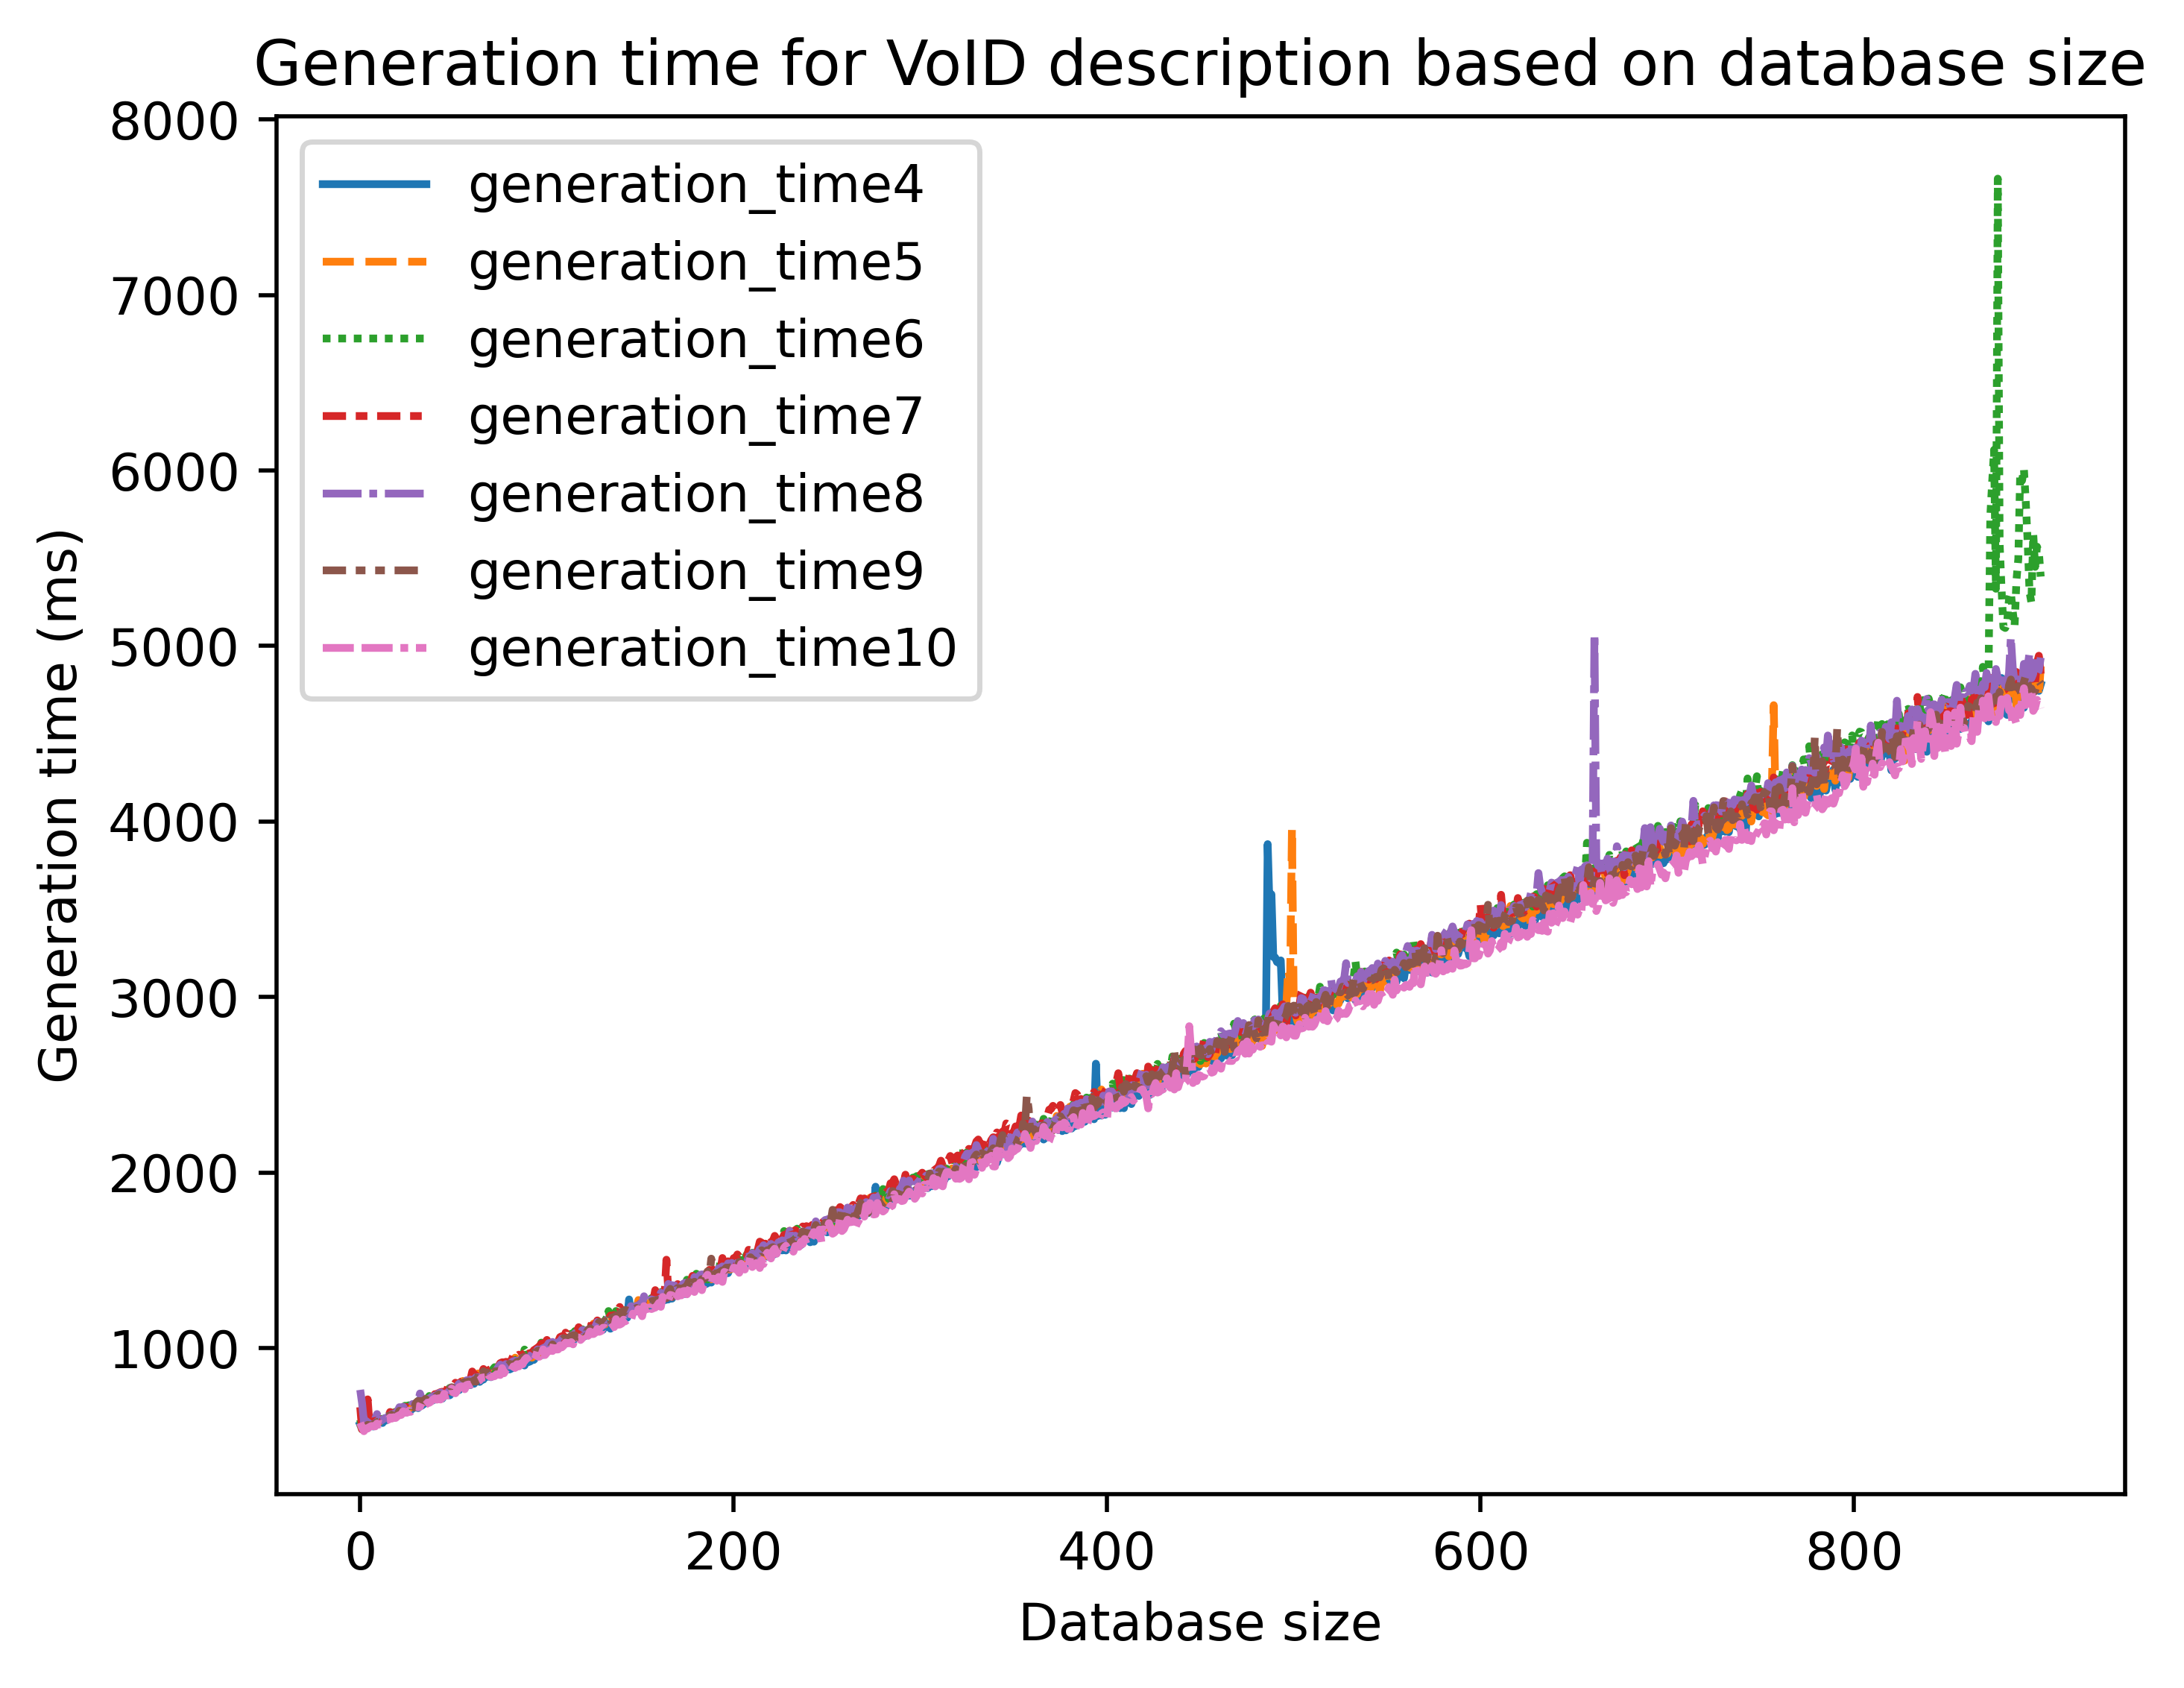
\includegraphics[width=0.8\columnwidth]{figures/generation-results-graph-all-good.png}
    \caption{2D graph showing each runs impact of database size on the time it takes to generate a VOID description. Containing only the good data.}
    \label{fig:generate-dbsize-10-runs-good}
\end{figure}